\documentclass[12pt,a4paper]{article}
\usepackage[utf8]{inputenc}
\usepackage[ngerman]{babel}
\usepackage[T1]{fontenc}
\usepackage{amsmath}
\usepackage{amsfonts}
\usepackage{amssymb}
\usepackage{graphicx}
\usepackage[left=2.5cm,right=2.5cm,top=2.5cm,bottom=3cm]{geometry}
\usepackage{multicol}
\usepackage{multirow}
\usepackage{hhline}
\usepackage{booktabs}
\usepackage[hidelinks]{hyperref}
\usepackage{tikz}
\usepackage{pgfplots}
\usepackage{blindtext}
\usepackage{array}
\usepackage{multirow}
\usepackage{bigdelim}
\usepackage{colortbl}
\usepackage{dblfloatfix}
% \usepackage{csquotes}
\usepackage{fancyhdr} 
\usepackage{kotex}
\usepackage{tabularx}
\usepackage{xcolor}
\usepackage{color}
\usepackage{tikzpeople} 
% \usepackage[backend=biber,style=alphabetic,]{biblatex} % TODO: Zeile Abklären und Löschen
\usepackage[backend=biber,style=numeric,]{biblatex}
\addbibresource{literatur.bib}
\setcounter{biburllcpenalty}{7000}
\setcounter{biburlucpenalty}{8000}
\usetikzlibrary{decorations.text}
\usetikzlibrary{tikzmark}
\usepackage{smartdiagram}
\usepackage[printonlyused]{acronym}
\usepackage[onehalfspacing]{setspace} 
\usepackage{float}
\usepackage{pdfpages}
\usepackage{enumitem}
\usepackage{calc}

\def\UrlBreaks{\do\/\do-}

\fancypagestyle{fancy}{
	\fancyhf{} 
	\fancyhead[L]{
\includegraphics[scale=0.028]{Bilder/dhbw_logo.png}} 
	\fancyhead[C]{T3\_2000}
	\fancyfoot[C]{\thepage}
}

\fancypagestyle{fancy_transition}{
	\fancyhf{} 
	\fancyhead[L]{
\includegraphics[scale=0.028]{Bilder/dhbw_logo.png}} 
	\fancyhead[C]{T3\_2000}
	\fancyfoot[C]{}
}

\fancypagestyle{titlepage}{
	\fancyhead[L]{} 
	\fancyhead[C]{} 
	\fancyhead[R]{}
	\fancyfoot[C]{}
}


\usepackage{helvet}
\renewcommand{\familydefault}{\sfdefault}

\urlstyle{same}
\author{\slshape Robin Rausch und Florian Maslowski}
\title{
\includegraphics[height=2.75cm]{Bilder/dhbw_logo.png}\vspace{2cm}\\\textbf{Planung und Entwicklung eines KI-Modells zum Transformieren von handschriftlichen Zeichnungen in fotorealistische Bilder}}
\pgfplotsset{compat=1.18}


\begin{document}
\pagestyle{titlepage}
\clearpage\maketitle
\thispagestyle{empty}
\vspace*{\fill}
\begin{center}
	\begin{tabularx}{\textwidth}{X X}
		Matrikelnummer & RR: 4718220 und FM: 2737788 \\
		Kurs & TINF21B \\
		Ausbildungsfirmen & Dürr Dental SE und Dürr Systems AG \\
		Ausbildungsorte & Bietigheim-Bissingen \\
		Betreuer & Prof. Dr.-Ing. Dipl. Inf. Kötter \\
	\end{tabularx}
\end{center}

\newpage
\pagenumbering{Roman}
\setstretch{1.5}

\pagestyle{fancy_transition}
\section*{Abstract}
\subsection*{Deutsch}
	Die Forschung im Bereich der künstlichen Intelligenz umfasst viele verschiedene Bereiche der Informationstechnik und Mathematik. 
	Aufgrund der aktuellen Entwicklungen und stetig fortschreitenden Forschung, ergeben sich immer mehr Möglichkeiten, diese Technologie anderswo einzusetzen.
	Die Arbeit beschäftigt sich mit der Planung und Entwicklung eines Modells basierend auf künstlicher Intelligenz, welches in der Kategorie Bild-zu-Bild einzuordnen ist. 
	Ziel der Arbeit ist ein funktionsfähiges Modell, das handgefertigte Zeichnungen und Skizzen in fotorealistische Bilder umwandeln kann. 
	Die Architektur dieses Modells soll aus bereits bestehenden Technologien konstruiert werden (Beispielsweise "Generative Adversarial Networks"). 
	Das Modell soll zur Kreativität und Inspiration bei Designprozessen verwendet werden können. 
	Ergebnis dieser Arbeit soll eine Applikation oder Website mit benutzerfreundlicher Oberfläche sein, welche das Erzeugen fotorealistischer Bilder anhand Skizzen ermöglicht. 
	Benutzer*innen können dann über eine auf der Oberfläche angezeigte Zeichenfläche Skizzen erstellen. 
	Diese werden dann in das zu erstellende Modell gegeben und das Ergebnis des Modells wird anschließend dem/der Benutzer*in angezeigt und zum Herunterladen angeboten. 
	Trainiert wird das Modell über ein zu erstellendes Datenset, welches aus bestehenden Daten aus dem Internet und selbst erzeugten Daten zusammengesetzt wurde. 

	Begonnen wird mit der Erstellung eines Datensatzes. 
	Hierzu werden Bilder aufgenommen und folglich als handgemalte Skizzen erstellt. 
	Zusätzlich werden Open-Source-Datensets aus dem Web verglichen und teilweise oder ganz übernommen. 
	Die Bilder werden dann in einem Datensatz zusammengefasst und später für das Trainieren des Modells verwendet. 
	Nebenher erfolgt eine ausführliche Recherche zur Thematik und speziell der verschiedenen Möglichkeiten der Architektur des Modells. 
	Darauf aufbauend soll die Struktur und allgemeine Planung des Modells erfolgen. 
	Nach Abschluss der Planung und Vorbereitung wird mit der Entwicklung des Modells begonnen. 
	Diese wird voraussichtlich in der Programmiersprache Python umgesetzt werden. 
	Zuletzt erfolgt die Implementierung des Modells in eine Applikation. 
	Zusätzlich wird eine Oberfläche erstellt, auf welcher Benutzer*innen Skizzen erstellen können und an das Modell gegeben werden. 
	Das resultierende Bild soll dann wieder ausgegeben werden.

\subsection*{Englisch}
	The research in the field of artificial intelligence encompasses many different areas of information technology and mathematics. 
	Due to current developments and ongoing research, more and more opportunities are emerging to apply this technology elsewhere.
	The work deals with the planning and development of a model based on artificial intelligence, which falls into the category of image-to-image. 
	The goal of the work is to create a functional model that can convert hand-drawn drawings and sketches into photorealistic images. 
	The architecture of this model is intended to be constructed from existing technologies, such as "Generative Adversarial Networks." 
	The model should be usable for fostering creativity and inspiration in design processes.
	The outcome of this work is expected to be an application or website with a user-friendly interface that allows the generation of photorealistic images based on sketches. 
	Users can create sketches on a drawing area displayed on the interface. These sketches are then input into the model to generate results, which are subsequently displayed to the user and made available for download.
	The model will be trained using a dataset to be created, composed of existing data from the internet and self-generated data. 
	The process begins with the creation of a dataset, where images are captured and subsequently transformed into hand-drawn sketches. 
	Additionally, open-source datasets from the web are compared and may be partially or fully incorporated. 
	The images are then compiled into a dataset and used for training the model.
	Simultaneously, comprehensive research on the subject matter and, specifically, the various architectural possibilities of the model is conducted. 
	Building upon this, the structure and general planning of the model will be developed. 
	After completing the planning and preparation, the model's development phase begins, which is likely to be implemented in the Python programming language. 
	Finally, the model is implemented into an application, and a user interface is created to allow users to create sketches and input them into the model. 
	The resulting image is then displayed again.

\newpage
\section*{Vorwort}
	Diese Arbeit entstand im Prozess des Absolvierens meines Dualen Studiums und handelt über \dots

\newpage
\section*{Ehrenwörtliche Erklärung}
	Ich erkläre hiermit ehrenwörtlich, dass ich die vorliegende Arbeit selbstständig und ohne Benutzung anderer als der angegebenen Hilfsmittel angefertigt habe. Aus den benutzten Quellen, direkt oder indirekt, übernommene Gedanken habe ich als solche kenntlich gemacht. Diese Arbeit wurde bisher in gleicher oder ähnlicher Form oder auszugsweise noch keiner anderen Prüfungsbehörde vorgelegt und auch nicht veröffentlicht.
	\vspace{1cm}
	\newline
	\noindent \raisebox{.2cm}{\rlap{\date{\today}, Bietigheim-Bissingen}}{\line(1,0){210}} \hfill \raisebox{.2cm}{\rlap{
\includegraphics[scale=.095]{Bilder/signature.png}}}{\line(1,0){200}}\\
	{\noindent \small Datum, Ort \hfill Unterschrift}

\newpage
\tableofcontents

\newpage
\pagestyle{fancy}
\phantomsection\addcontentsline{toc}{section}{Abkürzungsverzeichnis}
\section*{Abkürzungsverzeichnis}
\begin{acronym}
	\acro{udp}[UDP]{User Datagram Protocol}
	\acro{tcp}[TCP]{Transfer Control Protocol}
	\acro{ip}[IP]{Internet Protocol}
	\acro{osi}[OSI]{Open Systems Interconnection}
	\acro{sip}[SIP]{Session Initiation Protocol}
	\acro{api}[API]{Application Programming Interface}
	\acro{ai}[AI]{Artificial Intelligence}
	\acro{srtp}[SRTP]{Secure Real Time Transport Protocol}
	\acro{itut}[ITU-T]{International Telecommunication Union Telecommunication}
	\acro{vgl}[vgl.]{vergleiche}
	\acro{ki}[KI]{Künstliche Intelligenz}
	\acro{gan}[GAN]{Generative Adversarial Networks}
	\acro{vae}[VAE]{Variational Autoencoder}
	\acro{ki}[KI]{Künstliche Intelligenz}
	\acro{gpu}[GPU]{Graphics Processing Unit}
	\acro{cnn}[CNN]{Convolutional Neural Networks}
	\acro{relu}[ReLU]{Rectified Linear Unit}
	\acro{tanh}[Tanh]{Tangens hyperbolicus}
\end{acronym}

\newpage
\listoffigures
\vspace*{\fill}
%Was soll das?
% \hrule
% \begin{center}
% 	\small
% 	\begin{tabularx}{\textwidth}{l X}
% 		Deckblatt: & \url{https://upload.wikimedia.org/wikipedia/de/thumb/1/1d/DHBW-Logo.svg/2000px-DHBW-Logo.svg.png?20110626153129} \\
% 	\end{tabularx}
% \end{center}

\newpage
\pagenumbering{arabic}
\setstretch{1.5}
\acresetall

% Vorlagen:
%
% Beschreibungsbeispiel mit richtigem Abstand
% \begin{description}[leftmargin=!,labelwidth=\widthof{\bfseries UDP:}]
% 	\item[UDP:] Verbindungsloses Daten-streaming-Protokoll
% 	\item[TCP:] Verbindungsorientiertes Datentransferprotokoll  
% \end{description}
%
% Figur Beispiel
% \begin{figure}[H]
% 	\begin{center}
% 		\includegraphics[]{Bilder/...}
% 		\caption{Bildtitel}
% 		\label{img:beispiel}
% 	\end{center}
% \end{figure}
%
% Direktes Zitat: \cite[S.]{MITRE:Paper}. \\
% Indirektes Zitat: \cite[vgl.][S.322]{Book:ZeroDay}. \\
% Andere Quellenarten (siehe Quellen.bib Datei): \\
% Techreport: \cite{IEC:62443-4-2} \\
% Online: \cite{ESET:Industroyer}

\section{Einführung}
	% Zum Zeitpunkt des Schreibens dieser Arbeit ... \parencite[vgl.][]{assembly_in_dotnet}.\cite[vgl.][]{csharp_5.0_in_a_nutshell_page_3_to_5}
	In der heutigen Ära der künstlichen Intelligenz hat sich die Computerbildgebung zu einem dynamischen und faszinierenden Forschungsgebiet entwickelt. 
	Die Entwicklung von Algorithmen und Modellen zur Generierung von realistischen Bildinhalten aus unterschiedlichen Quellen ist zu einer bemerkenswerten Herausforderung geworden. 
	Dies ist insbesondere im Kontext der Transformationen von Handzeichnungen und Skizzen in fotorealistische Bilder von großer Bedeutung.
	Für diese Art von Bildtransformation soll das Modell "MAGIC" erschaffen werden.
	MAGIC steht für ''Marvelous AI for Generating Image Content'' und repräsentiert einen wichtigen Fortschritt in diesem Bereich.\\
	%
	Die Fähigkeit, aus handgezeichneten Skizzen fotorealistische Bilder zu erzeugen, ist nicht nur von technischem Interesse, sondern hat auch eine breite Palette von Anwendungen in Kunst, Design, Animation und sogar im Bereich der Medizin. 
	Diese Studienarbeit widmet sich der Entwicklung und Forschung von MAGIC und seiner Rolle bei der Umwandlung von Skizzen in eindrucksvolle und realistische Bildinhalte.\\
	%
	Im Verlauf dieser Arbeit werden wir einen detaillierten Blick auf die Funktionsweise von MAGIC werfen, die zugrundeliegenden Technologien und Algorithmen erforschen und verschiedene Anwendungsfälle beleuchten. 
	Darüber hinaus werden wir die Herausforderungen und Möglichkeiten in diesem Bereich erörtern, um ein umfassendes Verständnis für diese spannende Forschungsrichtung zu vermitteln.
	
\newpage
\section{Motivation}
\dots

\newpage
\section{Grundlagen}
	\subsection{Künstliche Intelligenz}
		Es ist schwer \ac{ki} genau zu definieren.
		Eine der verbreitetsten Definitionen geht aus der Arbeit ''Computing machinery and intelligence'' von Alan Turing hervor.
		Alan Turing war ein britischer Logiker, Mathematiker sowie Informatiker und Kryptoanalytiker. 
		In dieser Arbeit führte er den bekannten Turing Test durch, in welchem eine Maschine als intelligent eingestuft wird, wenn sie in einer Konversation nicht von einem Menschen unterschieden werden kann.
		\cite[\ac{vgl}][]{10.1111/bjd.18880}.
		% TODO: Turing test erklären

	\subsection{Maschinelles Lernen}
		Maschinelles Lernen bezieht sich auf Algorithmen und statistische Modelle, welche anhand eines Traingsdatensatzes bestimmte Muster erkennen oder Schlüsse ziehen.
		Um ein solches Modell zu trainieren, wird ein Teil des Traingsdatensatzes nicht zum Training sondern zum Testen verwendet wird.
		\cite[\ac{vgl}][S.424]{10.1111/bjd.18880}.\\
		%
		% TODO: Dimenstionsreduktion und Clusterbildung erklären
		Bei maschinellem Lernen wird zwischen verschiedenen Verfahren differenziert:
		%
		\begin{description}[leftmargin=!,labelwidth=\widthof{\bfseries Unüberwachtes Lernen:}]
			\item[Überwachtes Lernen:] Beim überwachten Lernen werden Algorithmen mit ausgewählten Trainingsdaten versorgt, die aus Eingabedaten und den zugehörigen Ausgabedaten bestehen. 
			Das Modell lernt, eine Assoziierung von Eingabe zu Ausgabe herzustellen. 
			Dies wird häufig für Aufgaben wie Klassifikation und Regression verwendet.
			\item[Unüberwachtes Lernen:]  Im unüberwachten Lernen werden Algorithmen mit Daten ohne vorherige Zuordnung oder Kennzeichnung trainiert. 
			Ziel ist es, verborgene Strukturen oder Muster in den Daten zu erkennen.
			Dazu werden beispielsweise Clusterbildungen oder Dimensionsreduktionen verwendet. 
			\item[Verstärktes Lernen:] Beim verstärkenden Lernen lernt ein Modell durch Interaktion mit seiner Umgebung. 
			Es erhält Feedback in Form von Belohnungen oder Bestrafungen und passt seine Aktionen an, um die Gesamtbelohnung zu maximieren. 
			Dieses Paradigma wird in Bereichen wie Robotik und Spieltheorie eingesetzt.
		\end{description}
		%
		Für das entwickeln eines intelligenten Modells ist Training sowie Testen essenziell.
		W3schools empfiehlt dafür den Datensatz in Trainings- und Testdaten aufzuteilen.
		Das Verhältnis wird mit 80\% für Trainingsdaten und 20\% für Testdaten angegeben \cite[\ac{vgl}][]{site:w3schoolstraintest}.
		%
		\subsubsection*{Anwendungen:}
			Das maschinelle Lernen findet in breitgefächerten Gebieten Anwendung.
			Aktuell wird es dazu verwendet, um in der Medizin neue Arzneimittel, Impfstoffe, etc. zu erschaffen.
			Außerdem wird es in Laboren für die Diagnose von Krankheiten und Viren verwendet.
			In der Wirtschaft wird maschinelles Lernen für die Risikobewertung, Aktienhandel, etc. verwendet.
			Ein Anwendungsgebiet, welches für diese Arbeit hohe Relevanz ist, ist die Bildverarbeitung.
			Dort wir maschinelles Lernen für Objekterkennung, Bildtransformationen, etc. verwendet.  

	\subsection{Deep Learning}
		Als Teilgebiet des maschinellen Lernens, wird bei dieser Art des Lernens auf den Nachbau eines menschlichen Gehirns gesetzt.
		Im menschlichen Gehirn befinden sich Neuronen/Gehirnzellen, welche miteinander verbunden sind. 
		Beim Anlernen neuen Wissens bilden sich neue Neuronenbindungen.
		Diese Verbindungen werden durch öftere Verwendungen gestärkt.
		Auf der anderen Seite werden selten genutzte Verbindungen schwächer, bis sie nicht mehr existent sind.
		Deep Learning Modelle versuchen dieses Prinzip nachzubauen.
		Dabei werden Neuronen durch Knotenpunkte repräsentiert, welche in mehreren Schichten/Layer angeordnet sind.
		Während dem Training werden die Gewichtungen der verschiedenen Verbindungen/Kanten mit dem Backpropagation-Prozess optimiert.
		Neuronale Netzwerke, welche über mehrere ''Hidden Layers'' verfügen, werden als ''deep'' neuronale Netze bezeichnet.
		\cite[\ac{vgl}][S.424]{10.1111/bjd.18880}
		%
		\begin{figure}[H]
			\begin{center}
				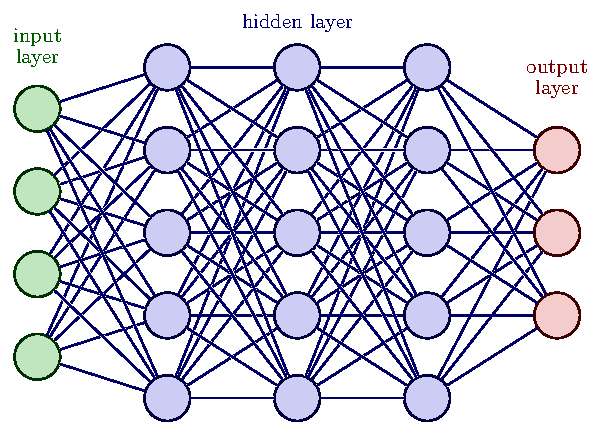
\includegraphics[width=0.9\textwidth, page=1]{Dateien/NeuralNetwork.pdf}
				\caption{Deep Learning Modell \cite[][]{site:neuralnetwork}}
				\label{img:deeplearning}
			\end{center}
		\end{figure}
		% TODO: Backpropagation
		Das Konzept des Deep Learnings war schon im Jahr 1943 bekannt.
		Ausschlaggebend dafür war der von Warren McCullough und Walter Pitts geschrieben Artikel ''A Logical Calculus of Ideas Immanent in Nervous Activity''.
		In diesem Artikel wurde erstmals das mathematische Modell eines neuronalen Netzwerks ausgearbeitet.
		1950 wurde ''Snarc'', der erste Computer mit neuronalem Netzwerk, von den Harvard-Studenten Marvin Minsky und Dean Edmonds erschaffen.
		Im selben Jahr hat auch Turing seine Arbeit ''Computing machinery and intelligence'', welche den Turing-Test beinhaltet, veröffentlicht \cite[\ac{vgl}][]{site:datascientestki}.
		%
		Jedoch war damals die Rechenleistung nicht ausreichend effizient und bezahlbar, um im Alltag Fuß zu fassen.
		Im Jahr 2013 wurde erkannt, dass Grafikkarten/\ac{gpu}, welche eigentlich für die Berechnung 3-Dimensionaler Grafiken in Computerspielen konzipiert waren, große Anwendung im repetitiven Training von neuronalen Netzwerken finden können.
		%
		\subsubsection*{\ac{cnn}} % TODO: CNN ausführen
			\ac{cnn} sind spezielle neuronale Netze, dessen Architektur besonders in der Bildverarbeitung als effektiv gilt.
			In den letzten Jahren stieg die Anzahl an Anwendungen aufgrund der demonstrierbaren Effizienz und Verfügbarkeit. 
			Unternehmen wie Google und Facebook investierten in die Entwicklung und Forschung dieser Netze.
			Daraus resultierten Architekturen, wie zum Beispiel Inception von Google und ResNet von Microsoft.
			Diese Architekturen können über Frameworks, wie TensorFlow und PyTorch für eigene Zwecke verwendet und weiterentwickelt werden.
			Ein häufiger Ansatz ist es vortrainierte Architekturen zu modifizieren, um individuelle Anwendungen zu meistern.\\
			%
			2017 wurde ein Meilenstein in der Medizin erreicht.
			Die Zuverlässigkeit eines \ac{cnn} konnte erstmals mit der eines Dermatologen verglichen werden.
			Für dieses Netzwerk wurde ein vortrainiertes Modell von Google für die medizinische Anwendung optimiert und mit einem eigenen Datensatz trainiert \cite[\ac{vgl}][]{10.1111/bjd.18880}.

	\subsection{Aktivierungsfunktionen}
		Im maschinellen Lernen werden Aktivierungsfunktionen verwendet, um Neuronen von neuronalen Netzen zu beeinflussen. 
		Sie skalieren und transformieren die Werte der Neuronen, bevor diese an die nächste Schicht des Netzwerks weitergeleitet werden. 
		Ohne diese Funktionen würde der Output nur eine lineare Funktion darstellen \cite[\ac{vgl}][]{site:activationfunctions}. 
		Neuronale Netze sind auch als „universelle Funktionsannäherungen“ bekannt, was heißt, dass sie jede Funktion erlernen können, welche als Input gegeben wird. 
		Mit der Hilfe von Aktivierungsfunktionen können deutlich komplexere Aufgaben, wie die Modellierung von Bildern, Videos, etc., umgesetzt werden. 
		Die Aktivierungsfunktionen müssen jedoch ableitbar sein, sodass eine Backpropagation implementiert und durchgeführt werden kann. 
		Die Backpropagation ist eine Optimierungsstrategie, welche die Fehler und Verluste in Bezug auf die Gewichte berechnet. 
		Diese Informationen werden für die Gewichtsoptimierung mittels Techniken wie das Gradientenabstiegsverfahren genutzt, um letztendlich die Ungenauigkeit im neuronalen Netzwerk zu reduzieren. 
		Das Gradientenabstiegsverfahren sucht nach dem globalen Minimum einer abgeleiteten Aktivierungsfunktion, um den Punkt mit der geringsten Fehlerquote zu finden \cite[\ac{vgl}][]{site:machinelearningautomation}.\\
		%
		Anhand folgender gängiger Aktivierungsfunktionen soll die Funktionsweise klar werden. 

		\subsubsection*{\ac{relu}}
			Die \ac{relu} ist eine der am häufigsten verwendeten Aktivierungsfunktionen in neuronalen Netzwerken. 
			Ihr grundlegender Ansatz besteht darin, alle negativen Eingaben auf null zu setzen und positive Eingaben unverändert zu lassen. 
			Die mathematische Darstellung von \ac{relu} lautet:
			\begin{align}
				Relu(x) = max(0,x)
			\end{align}
			\ac{relu} zeichnet sich durch seine Einfachkeit und Berechnungseffizients aus.
			Die Sparsity beschreibt einen hohen Anteil an Nullen oder nicht signifikanten Zahlen in einer Matrix. 
			Dies trägt zur effizienten Berechnung und Speicherung bei.
			Bei der Nullsetzung von negativen Werten, wird die Sparsity gefördert.
			Jedoch entsteht in der \ac{relu}-Funktion das ''Dead neurons Problem''. 
			Dabei werden Neuronen während des Trainings dauerhaft inaktiv. 
			Dies kann zu Informationsverlust führen und die Leistung des Netzwerks beeinträchtigen.\\
			\ac{relu} wird besonders in versteckten Schichten (englisch: hidden Layer) von tiefen neuronalen Netzen bevorzugt, da es dazu neigt, besser mit dem Vanishing Gradient Problem umzugehen. 
			In Anwendungen wie der Bilderkennung hat sich \ac{relu} als effektiv erwiesen, da es die Fähigkeit des Modells zur Extraktion von Merkmalen verbessert \cite[\ac{vgl}][]{9461312}.

		\subsubsection*{Sigmoid}
			Die Sigmoid-Aktivierungsfunktion ist eine nichtlineare Funktion, die im Bereich von 0 bis 1 liegt. 
			Dadurch transformiert die Aktivierungsfunktion Eingaben in diesen Wertebereich. 
			Sie wird oft in neuronalen Netzen für binäre Klassifikationsprobleme verwendet \cite[\ac{vgl}][]{9461312}.
			Die mathematische Darstellung von Sigmoid lautet:
			\begin{align}
				sig(x) = \frac{1}{1 + e^{-x}} 
			\end{align}
			Nachteilig ist bei dieser Funktion, die Neigung zum Vanishing Gradient Problem.
			Sigmoid findet daher typischerweise Anwendung in der Output-Schicht von neuronalen Netzwerken, um binäre Klassifikation zu ermöglichen. 
			Dabei gibt die Aktivierungsfunktion an, mit welcher Wahrscheinlichkeit ein bestimmtes Ereignis eintritt \cite[\ac{vgl}][]{site:machinelearningautomation}.

		\subsubsection*{\ac{tanh}}
			Die \ac{tanh} Funktion ähnelt der Sigmoid-Funktion, jedoch mit einem erweiterten Ausgabeumfang zwischen -1 und 1. 
			Dies führt dazu, dass die durch \ac{tanh} aktivierten Neuronen im Durchschnitt null ergeben, was das Training stabiler machen kann. 
			Diese Nullzentrierung, kann eine Voreingenommenheit des Modells mildern. 
			Die mathematische Darstellung von \ac{tanh} lautet:
			\begin{align}
				Relu(x) = max(0,x)
			\end{align}
			Die Nullzentrierung beugt außerdem dem Vanishing Gradient Problem in gewissem Maße vor und kann die Konvergenz in bestimmten Szenarien verbessern.
			In Aufgaben wie der Sprachverarbeitung und Textgenerierung hat sich \ac{tanh} als nützlich erwiesen \cite[\ac{vgl}][]{site:machinelearningautomation}.

		\subsubsection*{Wahl der Aktivierungsfunktion}
			Aus der Beschreibung der Aktivierungsfunktionen ergibt sich, dass es keine universell beste Funktion gibt, sondern jede Funktion ihre Vor- und Nachteile besitzt.
			Die Wahl der Aktivierungsfunktion hängt stark von den spezifischen Anforderungen der Anwendung ab.
			\ac{relu} bietet Effizienz und schnelle Konvergenz, während Sigmoid und \ac{tanh} in bestimmten Szenarien, wie binärer Klassifikation oder nullzentrierter Daten, ihre Stärken ausspielen.
			Es gibt aktuell noch viele weitere Aktivierungsfunktionen, welche in verschiedensten Anwendungsfällen geeignet sind. 
			Außerdem ist es möglich neue Aktivierungsfunktionen selbst zu entwickeln und zu erproben.

	\subsection{Generative Modelle}
		Generative Modelle zeichnen sich dadurch aus, Daten zu produzieren/generieren.
		Dabei wird anhand des Inputs, ein ''passender'' Output generiert.
		Die Qualität des Outputs hängt von mehreren Faktoren ab.
		Einige davon sind: % TODO: vervollständigen
		\begin{description}
			\item[Datenset:]
			\item[Verwendete Algorithmen:]  
			\item[Aktivierungsfunktionen:] ...
		\end{description}

	\subsection{Historie}

\newpage
\section{Problemstellung}
\dots

\newpage
\section{Evaluation generativer Modelle}
	\begin{figure}[H]
		\begin{center}
			\resizebox{\textwidth}{!}{
			\begin{tabular}{|c|c|c|c|c|}
				\hline
				\textbf{Modell} & \textbf{Bildqualität} & \textbf{Vielseitigkeit} & \textbf{Trainingszeit} & \textbf{Anwendungen} \\
				\hline
				GAN & Hoch & Vielseitig & Lang & Bildgenerierung \\
				\hline
				Pix2Pix & Hoch & Abhängig & Mittel & Bild-zu-Bild-Übersetzung \\
				\hline
				CycleGAN & Gut & Hoch & Mittel & Bild-zu-Bild-Übersetzung \\
				\hline
				VAE & Mittel & Mittel & Kurz & Bildgenerierung \\
				\hline
				SRGAN & Sehr hoch & Abhängig & Lang & Super-Resolution \\
				\hline
				Neural Style Transfer & Künstlerisch & Niedrig & Kurz & Stilübertragung \\
				\hline
				Diffusion Model & Hoch & Hoch & Lang & Vielseitige Anwendungen \\
				\hline
			\end{tabular}}
			\caption{Evaluationstabelle generativer Modelle}
			\label{img:evaluationstabellegm}
		\end{center}
	\end{figure}
	\begin{figure}[H]
		\begin{center}
			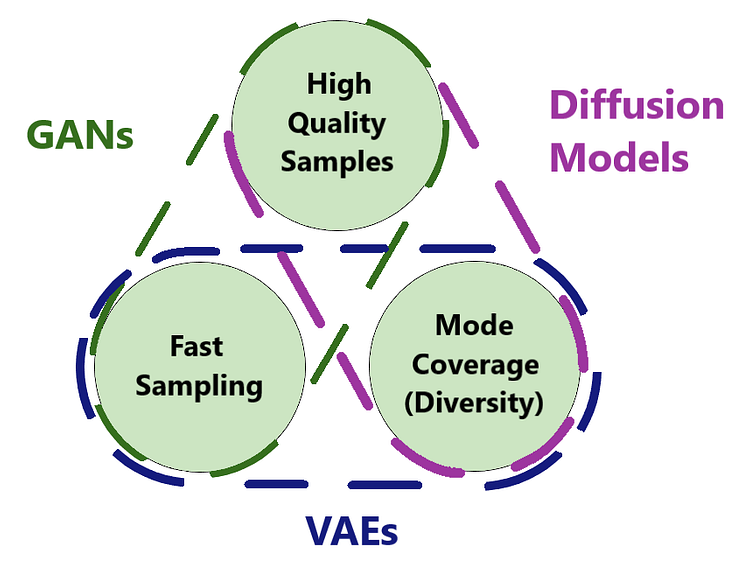
\includegraphics[width=0.5\textwidth]{Bilder/gan-diffusion-vae.png}
			\caption{Eigenschaften von \ac{gan}, \ac{vae} und Diffusion Modell}
			\label{img:propertiesganvaediffusion}
		\end{center}
	\end{figure}
	

	\subsection{\ac{gan}}

	\subsection{Diffusion}

\newpage
\section{Konzipierung}

\newpage
\section{Implementierung}

	\subsection{Datensatz erstellen}
		Der Datensatz soll in einer Datenbank gespeichert werden.
		Dafür wird eine Tabelle ''Datensatz'' mit den Spalten ''ID'', ''Foto'' und ''Skizze'' angelegt.
		Für die Zusammenstellung eines Datensatzes wurde ein Hilfsprojekt erstellt.
		In einer Oberfläche sollen Bilder angezeigt werden, welche der User abpausen kann.
		Nach fertigstellung der Skizzierung, kann diese in der Datenbanktabelle in der Spalte ''Sketches'' gespeichert werden.

	\subsection{Entwickeln eines generativen Modells}

		\subsubsection{Wahl der Aktivierungsfunktionen}
			- relu für hidden Layer.
			- Sigmoid oder Tanh für output layer
		
	\subsection{Aufsetzen der Infrastruktur}

\newpage
\section{Herausforderungen und Hindernisse}

\newpage
\section{Kritische Reflexion und Ausblick} 
	\subsection{Anwendungsgebiet}
		\subsubsection*{Design}
			Wird im Design Hilfe für den neuen Look eines Produkts benötigt, kann MAGIC, durch Generierung von kreativen Bildern, Inspiration bieten.
			Das Design kann auch vollständig übernommen werden.

		\subsubsection*{Animation}
			% TODO: Begründen warum Output jedes mal anders ist
			Im Bereich der Animation können durch simple Skizzen kreative Figuren erzeugt werden.
			Dennoch gilt es zu beachten, dass MAGIC keine vergangenen Skizzen mit ihren Ergebnissen speichert, weshalb das Modell in diesem Szenario in jeder Transformation unterschiedliche Ergebnisse generiert.
			Daher können keine Bilderreihen für Videos und Filme generiert werden.

		\subsubsection*{Kunst}
			In der Kunst kann das Modell ebenfalls für Inspiration oder sogar für die vollständige Ausarbeitung des Ergebnisses verwendet werden.
			Bei Änderung des Datensatzes zu größeren Kunstbilderanteilen, kann MAGIC für die Transformierung zu abstrakter oder konkreter Kunst optimiert werden. 

\newpage
\addcontentsline{toc}{section}{Literatur}
\small
\printbibliography	
\end{document}
